\documentclass[12pt,fleqn]{article}\usepackage{../common}
\begin{document}
Ders 15

Bu onemli bir ders, ana konumuz yansitma / projeksiyon (projection). Mesela
$b$ vektorunu alip $a$ uzerine olan ``yansimasini'' hesaplamak. 

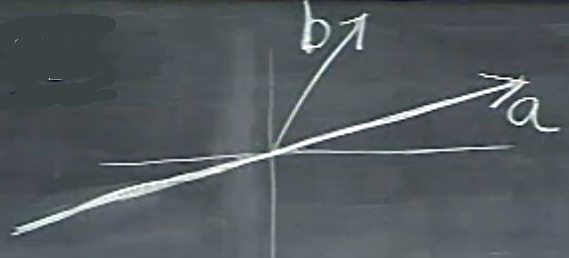
\includegraphics[height=2cm]{15_1.png}

Yansitmayi yapmak icin $b$'nin $a$'ya en yakin oldugu noktayi bulmaliyim. 

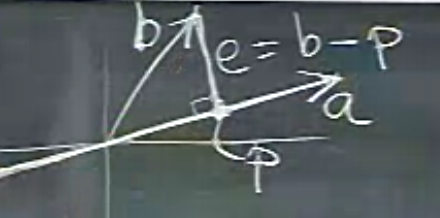
\includegraphics[height=2cm]{15_2.png}

Bu noktaya $p$ diyebilirim, $b,a$ arasindaki en kisa mesafeye de bir nevi
``hata (error)''  olarak bakabilirim, bu mesafeye $e$ harfini
verecegim. Hata sozunu kullandik, cunku, sanki $b$, $a$'dan ``sapmis'' ve
biz bu sapmanin olcusunu buluyoruz gibi bakilabilir bu probleme. 

Peki niye $e = b-p$? Su resme bakalim, 

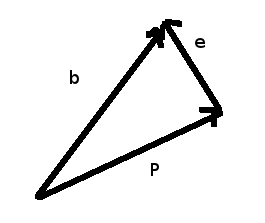
\includegraphics[height=3cm]{15_3.png}

Basit vektor aritmetiginden biliyoruz ki, birbirine zincirleme duran
vektorlerde, zincirin basindan sonuna direk gidilmek icin zincirdeki tum
vektorler birbiriyle toplanir. Ustteki resimde $b = p + e$. Ufak bir
cebirsel islemle $e = b - p$ buluruz. 

Peki $p$'yi nasil bulacagiz? Amacimiz bu, yansimayi bulmak. Muhakkak
elimizde bir dik ucgen var, eger trigonometri yapiyor olsaydik, cos, sin,
vs kullanip birseyler bulabilirdik. Lineer Cebir'in metotlari cok daha
temiz. 

Bildiklerimiz neler? Biliyoruz ki $p$, $a$'nin bir kati, cunku ayni cizgi
uzerindeler. 

\[ p = xa \]

diyelim. O zaman bulmak istedigim bu $x$ sayisi. 

Bildigimiz bir diger sey, $e$ ve $a$'nin birbirine dik oldugu. Iki vektorun
dik olmasinin tercumesi nedir? Iki vektorun noktasal carpiminin sifir
olmasi. O zaman

\[ a^T e = 0 \]

\[ a^T(b - p) = 0 \]

\[ a^T(b - xa) = 0 \]

Tekrar duzenlersem

\[ xa^Ta = a^Tb \]

Sol taraftaki $a^Ta$ bir tek sayi artik (cunku bir noktasal carpim), onu
alip sag tarafa bolum olarak tasiyabilirim,

\[ x = \frac{ a^Tb}{a^Ta} \]

Iste ihtiyacimiz olan katsayi bu. Bunun icinde cosine bir sekilde var
tabii, ama trigonometriye hic girmemize gerek yok, pur vektorler ile bu isi
hallettik. Sonra bu $x$'i alip $p = ax$ ile $p$'yi hesapliyoruz. Hepsini
biraraya koyarsak, 

\[ p = a\frac{ a^Tb}{a^Ta} \]

Biraz zihin egzersizi yapalim: eger $b$'yi iki katina cikarirsam, $p$ ne
olur? Iki katina cikar. Peki $a$'yi  iki katina cikarirsam? Ustteki resmi
dusunursek, hic degismemeli. Cebirsel olarak ta bunu gorebiliriz, ustteki
ve alttaki $a$'lardaki artis birbirini iptal edecektir. 

Simdi, olaya matrissel olarak bakmak gerekirse, bir yansitma matrisi $P$
olsun istiyorum, oyle ki 

\[ p = P b \]

olsun, yani bu matris $b$'ye uygulaninca $p$'yi bulayim. O zaman iki
ustteki $p$ formulu icinden $b$ haricindeki kisimlari cekip cikartmam
lazim.

\[ P  = \frac{ aa^T}{a^Ta} \]

Bu bir matris. Bolunen bir matris, bolen bir skalar. $P$ ilginc bir
matristir. Ozellikleri nedir? 

Kolon uzayi neydi? Bir vektoru o matris ile carptigimizda sonuc her zaman
matrisin kolon uzayindadir. $P$'nin kolon uzayi $a$'dan gecen cizgidir,
seviyesi (rank) 1'dir, simetriktir (bir vektoru devrigi ile sagdan carpinca
sonuc matrisi simetrik olur), yani $P^T = P$. 

Eger yansitma matrisini iki kere uygularsam ne olur? Ikinci yansitmanin
hicbir etkisi olmamasi gerekir, yani $P = P^2$. 

Eger daha yuksek boyutlara gecersek? O zaman ustune yansitma yaptigimiz bir
cizgi olmayacak, uc boyutta bir duzlem, daha yuksek boyutlarda N boyutlu
bir altuzay olacak.

Yansitma neye yarar? Onemli faydalarindan biri $Ax = b$ denklemini cozerken
ise yarar. Bazen bu denklemin cozumu yoktur. Belki bilinmeyenlerin sayisindan
daha fazla denklem verilmistir. O zaman tam denklemi cozmeye ugrasmak
yerine, cozulebilecek en yakin seyi cozmeye ugrasmak gerekir, yani 

\[ A\hat{x} = p \]

ki $p$, $b$'nin $A$'nin kolon uzayina yansitilmis hali olacak. Bir
``cozum'' olmak kolon uzayinin bir kombinasyonu olmak demek ise, bu kolon
uzayina yansitilan $b$ uzerinden cozumu elde edebilmeyi umabiliriz. 3
boyutta

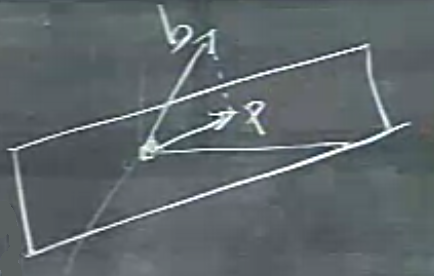
\includegraphics[height=3cm]{15_4.png}

Uzerine yansitma yapilacak duzlem nedir? Duzlemi belirlemek icin onu
tanimlayacak bir baz bulabilirim, iki vektor yani, mesela $a_1,a_2$
diyelim. 

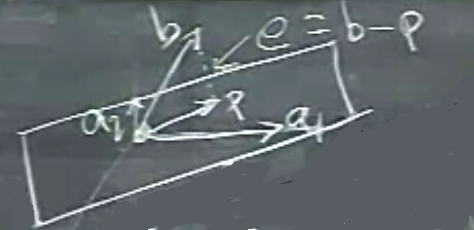
\includegraphics[height=3cm]{15_5.png}

Bu iki vektorun birbirine dik olmasi sart degil, bagimsiz olmasi gerekli
ama. $a_1,a_2$'nin yarattigi duzlem $A$'nin kolon uzayi ile aynidir, yani

\[ A = 
\left[\begin{array}{rr}
\uparrow &  \uparrow \\
a_1 &   a_2 \\
\downarrow &  \downarrow 
\end{array}\right]
 \]

$e$ duzleme diktir. Peki $p$ nedir? $a$ vektorlerinin bir kombinasyonudur, yani

\[ p = \hat{x}_1a_1 + \hat{x}_2a_2 \]

ya da daha temiz olarak

\[ p = A\hat{x} \]

Aradigimiz $\hat{x}$. Anahtar surada, $e$ yani 

\[  b - A\hat{x}\]

duzleme dik. Ve duzleme dik ise, duzlemdeki {\em her vektore} dik. O zaman 

\[ a_1^T( b - A\hat{x}) = 0\]

\[ a_2^T( b - A\hat{x}) = 0\]

Fakat ustteki gibi iki ayri formul yazmak yerine, matris formu kullanamaz
miyim? 

\[ 
\left[\begin{array}{rrr}
 & a_1^T & \\
 & a_2^T & 
\end{array}\right]
(b - A\hat{x}) = 
\left[\begin{array}{rrr}
0 \\
0 
\end{array}\right]
 \]

Ya da

\[ A^T(b - A\hat{x})  = 0 \]

Bu problemin cizgizel versiyonunde $A$ yerine $a$ kullanmistik, ve $a$ tek
bir vektordu. Zaten $A$ yerine $a$ kullanirsak, ayni formulu elde
ediyoruz. 

Bir soru soralim simdi: $e$, yani $b - A\hat{x}$ hangi uzayin icindedir?
Cevap, $A^T$'nin sifir uzayindadir (nullspace), yani $N(A^T)$ icinde. Sifir
uzayi hakkinda neler biliyoruz? Sifir uzayi ve kolon uzaylari birbirine
ortogonaldir. O zaman $e$  $N(A^T)$ icinde ise, $e \perp C(A)$ demektir,
yani $e$ de kolon uzayina ortogonaldir. Devam edelim, ustteki formulu duzenlersek,

\[ A^TA\hat{x} = A^Tb \]

Dikkat edersek, onceki versiyonda $a^Ta$ bir tekil sayiydi, boylece onu
bolen olarak saga gecirmistik. Simdi ne yapacagiz? 

\[ \hat{x} = (A^TA)^{-1}A^Tb \]

Daha once 

\[ p = A\hat{x} \]

demistik, o zaman 

\[ p = A(A^TA)^{-1}A^Tb \]

Demek ki yansitma matrisi esitligin saginda $b$ harici olan tum semboller, 

\[ P = A(A^TA)^{-1}A^T \]

Simdi dikkat, bilerek bir hata yapacagim, ustteki formulun sag tarafini
cebirsel olarak manipule edecegim

\[  AA^{-1}(A^T)^{-1}A^T = I\]

Bu yanlis duruyor, $P$ birim matris olamaz. Nerede hata yaptik?
Manipulasyon mekanik, teknik olarak dogru. Hata $A$'nin kare matrisi
olmamasinda. O sebeple $A^TA$'yi ustte yaptigim gibi parcalayamam cunku
bir matrisin tersini alabilmek icin onun en azindan kare olmasi gerekir (bu
yeterli sart degil tabii ki). 

Yansima matrislerinin simetrik olmasini bekliyordum, ve bakiyorum ki oyle. 

\[ P^T = P \]

ve 

\[ P^2 = P \]

Kontrol edelim

\[=  A(A^TA)^{-1}A^T \ A(A^TA)^{-1}A^T \]

\[=  A(A^TA)^{-1}\cancel{A^T \ A(A^TA)^{-1}}A^T \]

\[=  A(A^TA)^{-1}A^T \]

Ustteki son ifade $P$'ye esit. 

Uygulama: En Az Kareler (Least Squares)

Ne zaman formulden daha fazla veri vardir? Mesela veriye cizgi ``uydurmak
(fitting)'' istedigimde durum budur. Diyelim ki $t,D$ eksenleri uzerinde

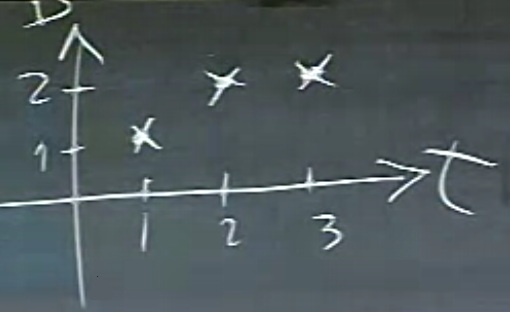
\includegraphics[height=3cm]{15_6.png}

Veri soyle olsun, $(1,1),(2,2),(3,2)$, uc tane nokta. Bu noktalara en yakin
sekilde gececek cizgi kabaca soyle olur [cizgi pek duz olmadi ama neyse].

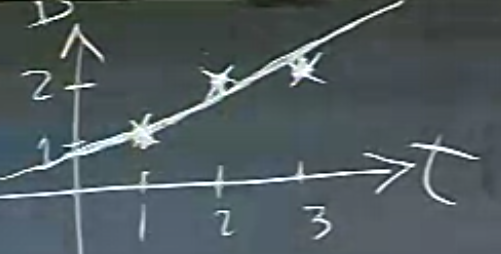
\includegraphics[height=3cm]{15_7.png}

Bu problem odevde $b = C+Dt$ olarak gosterildi. O zaman 

\[ C + D = 1 \]

\[ C + 2D = 2 \]

\[ C + 3D = 2 \]

Bu tur problemleri cozerken anahtar yaklasim bu, formulu yazalim, ve cozmek
istedigimiz (ama cozemedigimiz) denklemler serisini ortaya
cikaralim. Matris olarak yazarsak, 

\[ 
\underbrace{
\left[\begin{array}{rr}
1 & 1 \\
1 & 2 \\
1 & 3 
\end{array}\right]
}_{A}
\underbrace{
\left[\begin{array}{r}
C  \\
D  
\end{array}\right]
}_{x}
=
\underbrace{
\left[\begin{array}{r}
1 \\
2 \\
2  
\end{array}\right]
}_{b}
 \]

Gordugumuz gibi 3 tane denklem ve 2 tane bilinmeyen var. Yani verilen
(denklemler) bilinmeyenlerden daha fazla. Bu sebeple bazi denklemler (ya da
hicbiri) dogal olarak tam olarak uymayacak. Amac $Ax = b$'yi cozmek degil,
yansimayi cozmek. O zaman $A$'yi alttaki yerine koyunca, cozum ortaya
cikacaktir. 

\[ \hat{x} = (A^TA)^{-1}A^Tb \]




\end{document}
